\documentclass[11pt]{article}


\usepackage{preamble}

\title{Error Correcting Codes, Hardness Amplification and Boosting.}
\date{}

\begin{document}
    
\noindent Error Correcting Codes, Hardness Amplification and Boosting \hfill  CS 250, Winter 2025\\
\hrule


\section{Introduction}

The purpose of this paper is to discuss the connection between three different topics in theoretical computer science: error correcting codes, hardness amplification,

%\tableofcontents

\section{Hardness Amplification with ECCs}

This section will discuss the connection between error correcting codes and hardness amplification. In particular, we'd like to understand the relationship between three different assumptions, which we list below. The first is the worst case hardness assumption, which says that there exists a function computable in exponential time which nonetheless cannot be computed \emph{exactly} by somewhat large circuits.

\begin{assumption}{1}[Worst Case Hardness] \label{a-1}
    There exists a function $f : \pmon \rightarrow \pmo$ such that $f$ can be computed in time $2^{O(n)}$, but there exists some constant $\delta > 0$ such that 
    \begin{equation*}
        \Corr\left(f, 2^{\delta n}\right) < 1.
    \end{equation*}
\end{assumption}

Mild hardness strengthens this slightly: instead of asking that any circuit attempting to compute $f$ errs on at least $1$ input, we ask that it messes up on a constant fraction (say 90\%) of inputs.

\begin{assumption}{2}[Mild Hardness] \label{a-2}
    There exists a function $f : \pmon \rightarrow \pmo$ such that $f$ can be computed in time $2^{O(n)}$, but there exists some constant $\delta > 0$ such that 
    \begin{equation*}
        \Corr\left(f, 2^{\delta n}\right) < .9.
    \end{equation*}
\end{assumption}

Finally, average case hardness strengthens both of the above by a large margin, requiring that any small circuit attempting to compute $f$ cannot get better than exponentially small correlation.

\begin{assumption}{3}[Average Case Hardness] \label{a-3}
    There exists a function $f : \pmon \rightarrow \pmo$ such that $f$ can be computed in time $2^{O(n)}$, but there exists some constant $\delta > 0$ such that 
    \begin{equation*}
        \Corr\left(f, 2^{\delta n}\right) < 2^{-\Omega(n)}.
    \end{equation*}
\end{assumption}

To see just how strong of an assumption this is, consider that for any $f$, the algorithm which just randomly guesses the output achieves correlation $0$ with $f$; thus, \hyperref[a-3]{Assumption 3} supposes that an explicit function exists which even exponentially large circuits cannot compute much better than random guess. Clearly, \hyperref[a-3]{Assumption 3} implies \hyperref[a-2]{Assumption 2}, and \hyperref[a-2]{Assumption 2} implies \hyperref[a-1]{Assumption 1}; but can we go in the opposite direction? Given a function which large circuits cannot compute exactly, can we construct a function which large circuits cannot compute much better than random guessing? Surprisingly, the answer is yes.

\begin{theorem}{2.1}[\cite{iw97}, \cite{STV99}]\label{t-2-1}
    If there exists a function $f$ satisfying the worst case hardness assumption, there exists a function $f'$ satisfying the average case hardness assumption.
\end{theorem}

Before proving this, however, we will discuss why we care about hardness amplification, and why we'd like to find a function satisfying \hyperref[a-3]{Assumption 3}.

\subsection{Why Hardness Amplification?}

While hardness amplifcation is useful in other fields such as cryptography, in this section we will focus on its applications to psuedorandomness. In particular, we will discuss how to use average case hard functions to construct good \emph{psuedorandom generators}, a special type of function which maps a small number of truly random bits to a large number of psuedorandom bits. Here, by ``pseudorandom'' bits, we mean a string of bits which computationally bounded programs cannot distinguish from truly random bits.

\begin{definition}{2.1}
    We say that a function $G : \pmo^\ell \rightarrow \pmo^{n}$ is an $(\ell, n)$-PRG if, for any size $n$ circuit $C$ over $n$ inputs, 
    \begin{equation*}
        \left|\Pr_{x \backsim U_n}[C(x)] - \Pr_{s \backsim U_\ell}[C(G(s))]\right| < \frac{1}{10}.
    \end{equation*}
    We will call $\ell$ the \emph{seed length} of $G$.
\end{definition}

The definition above says that up to a small (i.e., $\sfrac{1}{10}$) difference, the generator $G$ ``fools'' any small circuit into believing it's output is truly random. Why are we interested in psuedorandom generators? The theorem below demonstrates that, given an efficient to compute PRG which has relatively small seed length, any efficient \emph{randomized} algorithm for a problem can be converted into an efficient \emph{deterministic} algorithm.


\begin{theorem}{2.2} \label{t-2-2}
    Suppose that $G$ is a $(O(\log n), n)$-PRG computable in $\poly(n)$ time. Then $\P = \BPP$.
\end{theorem}

Given that it is unknown whether $\P = \BPP$, it should be clear that we don't know whether such PRGs exist. However, in 1994 Nisan and Wigderson \cite{NW94} gave an elegant connection between the existence of hard functions and the existence of good psuedorandom generators.

\begin{theorem}{2.3}[Nisan-Wigderson Generator, \cite{NW94}] \label{t-2-3}
    Given the average case hardness assumption (\hyperref[a-3]{Assumption 3}), there exists a $(O(\log n), n)$-PRG.
\end{theorem}

Thus, given an average case hard function we can construct a good psuedorandom generator, and given this good psuedorandom generator we can efficiently derandomize $\BPP$. This gives us a promising new avenue to generically derandomize algorithms; however, it seems extremely difficult to prove that a function is average case hard. We can reduce this burden by amplifying hardness, meaning we only need to prove worst case hardness for a particular function to construct good PRGs. In other words, taking some function which is computable in exponential time and is believed to be hard (i.e., $\SAT{}$), we can combine Theorems \hyperref[t-2-1]{2.1}, \hyperref[t-2-2]{2.2}, and \hyperref[t-2-3]{2.3} to show that proving worst case lower bounds suffices to derandomize $\BPP{}$.

\begin{corollary}{2.1}
    If there exists some $\delta > 0$ such that \SAT{} requires circuits of size $\Omega(2^{\delta n})$, then $\P = \BPP$.
\end{corollary}

The remainder of this section will outline the connection between hardness and randomness, demonstrating how can convert hard functions into good PRGs.

\subsubsection{A Simple PRG}

To see the key ideas used in constructing a PRG capable of derandomizing BPP, we will use the average case hardness assumption to construct a PRG which increases the size of the pseudorandom string by one bit. While such a PRG is not very useful for derandomization, the analysis in this section will be helpful when we construct our stronger PRG.

\begin{theorem}{2.4}[\cite{NW94}]\label{t-2-4}
    Given the average case hardness assumption, there exists a $(n - 1, n)$-PRG.
\end{theorem}
\noindent
Have $f : \pmo^{n - 1} \rightarrow \pmo$ be an average case hard function. Our $(n - 1, n)$-PRG $G$ will be defined as follows:
\begin{equation*}
    G(s_1, \ldots, s_{n - 1}) = \bigl(s_1, \ldots, s_{n - 1}, f(s_1, \ldots, s_{n - 1})\bigr).
\end{equation*}
In this case, the first $n - 1$ bits are truly random, and so no circuit will be able to distinguish them from uniform random bits. For the last bit, since any small circuit can't do much better than guessing the value of $f$, this bit will also appear essentially random. To formalize this, we will use Yao's next bit prediction lemma. Intuitively, it reduces the task of analyzing a circuit's behavior on an entire psuedorandom string to analyzing it's ability to predict a particular bit given the previous bits.
\begin{lemma}{2.1}[Yao's next bit prediction lemma, \cite{Yao82}]\label{l-2-1}
    Write $G(s) = (z_1, \ldots, z_n)$. Suppose that for all $i \in [n]$, any circuit $C : \pmo^{i - 1} \rightarrow \pmo$ of size $n$ has 
    \begin{equation*}
        \Corr\left(C(z_1, \ldots, z_{i - 1}), z_i\right) < \frac{\epsilon}{n}. \tag{1}
    \end{equation*}
    Then for any $C : \pmo^n \rightarrow \pmo$ of size $n$, 
    \begin{equation*}
        \left|\Pr_{x \backsim U_n}[C(x)] - \Pr_{s \backsim U_\ell}[C(G(s))]\right| < \epsilon. \tag{2}
    \end{equation*}
\end{lemma}
Note that fixing $\epsilon = \sfrac{1}{10}$, the condition in equation (2) says that $G$ is a $(n - 1, n)$-PRG. Thus, to prove  \hyperref[t-2-4]{Theorem 2.4}, we just need to show that $G$ satisfies the hypothesis of \hyperref[l-2-1]{Lemma 2.1}: the $i$-th bit should be unpredictable given the first $i - 1$ bits.

\begin{proof}[Proof \textup{(Of \hyperref[t-2-4]{Theorem 2.4})}.]
    By \hyperref[l-2-1]{Lemma 2.1}, it suffices to show that for any $i \in [n]$ and circuit $C$ of size $n$, 
    \begin{equation*}
        \Corr(C(z_1, \ldots, z_{i - 1}), z_i) < \frac{1}{10 n}. \tag{3}
    \end{equation*}
    First, see that for $i \in [n - 1]$, the bit $z_i$ is independent of the first $i - 1$ bits. Thus, $z_i$ is independent of the output of $C$, and so the correlation must be equal to $0$. When $i = n$, we can expand the expression with our definition of $G$,
    \begin{equation*}
        \Corr(C(z_1, \ldots, z_{n - 1}), z_n) = \Corr(C(z_1, \ldots, z_{n - 1}), f(z_1, \ldots, z_{n - 1})) = \Corr(C, f).
    \end{equation*}
    Now, since $C$ is a size $n$ circuit, while $f$ is average case hard against size $2^{\delta (n - 1)} = O(2^{\delta n})$ size circuits,
    \begin{equation*}
        \Corr(C, f) \leq 2^{-\Omega(n - 1)} < \frac{1}{10 n}.
    \end{equation*}
    Thus, equation (3) holds for all $i \in [n]$, and so $G$ is a $(n - 1, n)$-PRG.
\end{proof}

\subsubsection{The Nisan-Wigderson Generator}

Extending the analysis above, Nisan and Wigderson \cite{NW94} used the average case hardness assumption to construct a pseudorandom generator stretching the seed bits exponentially further.

\begin{theorem}{2.5}[Nisan-Wigderson Generator, \cite{NW94}]
    Given the average case hardness assumption, there exists a $(O(\log n), n)$-PRG.
\end{theorem}

\noindent
The generator works by having \emph{every} bit of the output compute the hardcore function on ``roughly disjoint'' subsets of the bits of the seed $s \in \pmo^{O(\log n)}$. To demonstrate the construction, we will fix some constant $c > 1$ which we are free to choose later and have $f$ be an average case hard function such that $\Corr(f, 2^{\delta n}) < 2^{-\delta n}$. Given any collection $\cS$ of $n$ subsets $S_1, \ldots, S_n \subseteq [c \log n]$, each of size $\sfrac{2}{\delta} \cdot \log n$, we can construct a generator $G_\cS$ as follows: given a seed $s \in \pmo^{c \cdot \log n}$, the $i$-th output of $G_\cS$ will correspond to the evaluation of $f$ on the subset of bits $S_i$,
\begin{equation*}
    (G_\cS(s))_{i} = f(s_{j_1}, \ldots, s_{j_{\sfrac{2}{\delta} \cdot \log n}}), \quad \left\{j_1, \ldots, j_{\sfrac{2}{\delta} \cdot \log n}\right\} = S_i.
\end{equation*}
As a picture, our psuedorandom generator $G_\cS$ looks something like this.
\begin{center}
    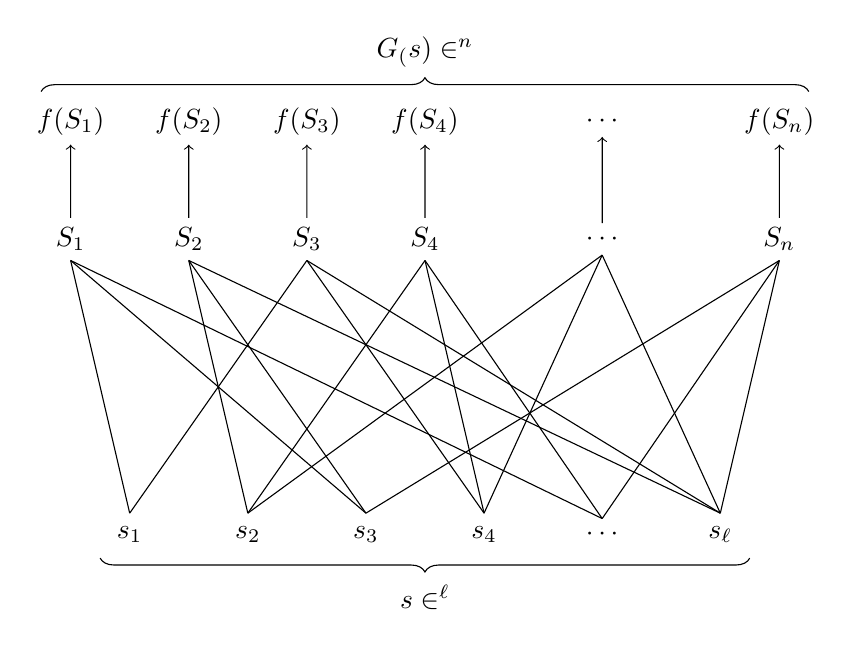
\begin{tikzpicture}[align=center,node distance=4cm, scale=1.5]
        \node[circle, inner sep=0pt, minimum size=15pt] (1) at (1, 0) {$s_1$}; 
        \node[circle, inner sep=0pt, minimum size=15pt] (2) at (2, 0) {$s_2$};
        \node[circle, inner sep=0pt, minimum size=15pt] (3) at (3, 0) {$s_3$};
        \node[circle, inner sep=0pt, minimum size=15pt] (4) at (4, 0) {$s_4$};
        \node[] (5) at (5, 0) {$\cdots$};
        \node[circle, inner sep=0pt, minimum size=15pt] (6) at (6, 0) {$s_{\ell}$};

        \node[] (11) at (.5, 2.5) {$S_1$};
        \draw[] (1.north) -- (11.south);
        \draw[] (3.north) -- (11.south);
        \draw[] (5.north) -- (11.south);

        \node[] (21) at (.5, 3.5) {$f(S_1)$};

        \draw[->] (11) -- (21);


        \node[] (12) at (1.5, 2.5) {$S_2$};
        \draw[] (2.north) -- (12.south);
        \draw[] (3.north) -- (12.south);
        \draw[] (6.north) -- (12.south);

        \node[] (22) at (1.5, 3.5) {$f(S_2)$};

        \draw[->] (12) -- (22);


        \node[] (13) at (2.5, 2.5) {$S_3$};
        \draw[] (1.north) -- (13.south);
        \draw[] (4.north) -- (13.south);
        \draw[] (6.north) -- (13.south);

        \node[] (23) at (2.5, 3.5) {$f(S_3)$};

        \draw[->] (13) -- (23);


        \node[] (14) at (3.5, 2.5) {$S_4$};
        \draw[] (2.north) -- (14.south);
        \draw[] (4.north) -- (14.south);
        \draw[] (5.north) -- (14.south);

        \node[] (24) at (3.5, 3.5) {$f(S_4)$};

        \draw[->] (14) -- (24);


        \node[] (15) at (5, 2.5) {$\cdots$};
        \draw[] (4.north) -- (15.south);
        \draw[] (2.north) -- (15.south);
        \draw[] (6.north) -- (15.south);

        \node[] (25) at (5, 3.5) {$\cdots$};

        \draw[->] (15) -- (25);

        \node[] (16) at (6.5, 2.5) {$S_n$};
        \draw[] (3.north) -- (16.south);
        \draw[] (5.north) -- (16.south);
        \draw[] (6.north) -- (16.south);

        \node[] (26) at (6.5, 3.5) {$f(S_n)$};

        \draw[->] (16) -- (26);

        \draw [decorate,decoration={brace,amplitude=5pt}]
  (0.25,3.75) -- (6.75,3.75) node[midway, yshift=.5cm]{$G_\cS(s) \in \pmo^{n}$};

        \draw[decorate, decoration={brace,amplitude=5pt, mirror}] 
        (.75, -.2) -- (6.25, -.2) node[midway, yshift=-.5cm]{$s \in \pmo^{\ell}$};
    \end{tikzpicture}
\end{center}
\noindent
The key to creating a good psuedorandom generator is picking a good collection of subsets $\cS$, and to do that, we need to explain what we mean by ``roughly disjoint'' subsets. The reason why we can't just take any collection of subsets is that, if two distinct subsets $S_i$ and $S_j$ overlap too much, then the $i$-th and $j$-th bits of $G_\cS$ will be very correlated, preventing us from using Yao's next bit prediction lemma in our analysis. On the other hand, if we wanted to make each subset truly disjoint, the seed length of our PRG $G_\cS$ would be at least $\sfrac{2}{\delta} \cdot n \cdot \log n = O(n \log n)$, making this a terrible PRG.

Thus, we need to choose $\cS$ to balance between these two extremes: we need some overlap so that the seed length is small, but not too much that different bits in the output are very correlated. As it turns out, the following requirements will suffice for $G_\cS$ to be a good PRG:
\begin{enumerate}
    \item $\cS$ contains $n$ subsets $S_1, S_2, \ldots, S_n \subseteq [c \log n]$,
    \item every subset $S_i$ has size $|S_i| = \sfrac{2}{\delta} \cdot \log n$,
    \item for distinct $i \neq j$, $|S_i \cap S_j| \leq \log n$.
\end{enumerate}
Initially, it is not obvious that such a collection $\cS$ exists: can we even find an exponential (in $\log n$) number of subsets of $O(\log n)$ bits, each of size $O(\log n)$, which have overlap at most $\log n$? As it turns out, objects satisfying these properties have a name: a collection $\cS$ satisfying properties 1-3 is called a $(c \log n, \sfrac{2}{3} \cdot \log n, \log n, n)$-\emph{combinatorial design}. Moreover, for a large enough constant $c > 1$, such combinatorial designs exist.

\begin{lemma}{2.2}[Existence of combinatorial designs, \cite{NW94}]\label{l-2-2}
    There exists a constant $c > 1$ such that a $(c \log n, \sfrac{2}{3} \cdot \log n, \log n, n)$-combinatorial design exists and can be produced in $\poly(n)$ time.
\end{lemma}

While we will not go through the analysis here, one can prove \hyperref[l-2-2]{Lemma 2.2} with the natural greedy algorithm: start with an empty collection $\cS$ and iterate through all subsets of size $\sfrac{2}{\delta} \cdot \log n$, adding any subset to $\cS$ which does not overlap too much with the subsets already added to $\cS$. 

Thus, combining \hyperref[l-2-2]{Lemma 2.2} with \hyperref[a-3]{Assumption 3} using our construction above, $G_\cS$ will be a $(O(\log n), n)$-PRG. In sum, we can construct good PRGs from average case hard functions, allowing us to use such an assumption to derandomize \BPP{}.

\subsection{Worst Case Hardness to Mild Hardness}

Now that we've completed our discussion of the connection between average case hard functions and psuedorandom generators, we will move on to the the actual task of hardness amplification. To see the essential connection between hardness amplification and error correcting codes, we will start by proving that we can convert worst case hard functions into mildly hard functions given an error correcting code $\cC$ which is locally decodable; in the following section, we will work through actually constructing such a code.

\begin{theorem}{2.6}\label{t-2-6}
    Suppose that $\cC$ is a $[m^2, m]_2$ code with the following properties: (1) the encoding map $\Enc : \pmo^m \rightarrow \pmo^{m^2}$ is computable in $\poly(m)$ time, and (2) there exists a local decoding algorithm $\LDec$ which can correct up to a relative distance of $.05$ running in $\polylog(m)$ time. Then the worst case hardness assumption implies the mild hardness assumption.
\end{theorem}

\begin{proof}

    Suppose that there exists a function $f : \pmon \rightarrow \pmo$ which can be computed in time $2^{O(n)}$ but, for some $\delta > 0$, 
    \begin{equation*}
        \Corr\left(f, 2^{\delta n}\right) < 1.
    \end{equation*}
    Having $N = 2^n$, we can represent $f$ as a string of length $N$ by its truth table $\TT(f) \in \pmo^N$. Then when we encode this string using our code $\cC$, we can view the string $\Enc(\TT(f)) \in \pmo^{2N}$ as the truth table of a function $\TT(\hat{f})$, where $\hat{f} : \pmo^{2n} \rightarrow \pmo$. We claim that for some constant $\delta' > 0$,
    \begin{equation*}
        \Corr\left(\hat{f}, 2^{\delta' n}\right) \leq .9.
    \end{equation*}
    To prove this, suppose for the sake of contradiction that there existed a circuit $C$ of size $2^{\delta' n}$ with correlation $\geq .9$ with $\hat{f}$. We will use $C$ to construct a circuit perfectly computing $f$. To start, consider the truth table $\TT(C)$ of the function computed by $C$. Because $C$ achieves high correlation with $\hat{f}$, the relative distance between $\TT(C)$ and $\TT(\hat{f})$ must be small, $\delta\left(\TT(C), \TT(\hat{f})\right) < .05$. Thus, if we give our local decoder $\LDec$ for $\cC$ query access to $\TT(C)$, it will with probability $\sfrac{2}{3}$ output any particular bit of $\TT(f)$ in $\polylog(N) = \poly(n)$ time. Consider the following randomized circuit $C_{\sfrac{2}{3}}$ which computes $f$ with probability $\sfrac{2}{3}$. On input $x \in \pmon$, run the local decoder on $x$, simulating query access to $\TT(C)$ by querying the circuit $C$ itself,
    \begin{equation*}
        C_{\sfrac{2}{3}}(x) = \LDec^{\TT(C)}(x).
    \end{equation*}
    The size of $C_{\sfrac{2}{3}}$ depends on the running time and query complexity of $\LDec$, since each query to $\TT(C)$ is simulated by an independent copy of $C$. Since both of these quantities are $\poly(n)$, we see that 
    \begin{equation*}
        |C_{\sfrac{2}{3}}|  \leq \poly(n) + \poly(n) |C| \leq 2^{(\delta' + o(1))n}.
    \end{equation*}
    Using the fact that circuits can be derandomized with only a polynomial blow up in size, we can obtain a circuit $C'$ of size $2^{(\delta' + o(1))n}$ compute $f$ exactly. Taking $\delta' = \delta / 3$, this would contradict the fact that $f$ cannot be computed exactly by circuits of size $2^{\delta n}$. Thus, it must be true that 
    \begin{equation*}
        \Corr\left(\hat{f}, 2^{\delta n / 3}\right) \leq .9.
    \end{equation*}
    The last thing we must verify is that $\hat{f}$ can still be computed in time $2^{O(n)} = \poly(N)$. Since our encoding map $\Enc$ and $f$ are both computable in $\poly(N)$ time, $\hat{f}$ will be as well.
\end{proof}

\subsubsection{Reed-Muller and Hadamard Codes}

\hyperref[t-2-6]{Theorem 2.6} reduces the task of hardness amplification to finding a suitable error correcting code. The most important property of this code is that it is locally decodable. As a starting point, let's take a look at a code which has good rate, distance and is locally correctable: the Reed-Muller code.

\begin{definition}{2.2}[Reed-Muller Codes]
    Suppose $\F$ is a finite field of size $q$. The Reed-Muller code $\RM_q(m, d)$ is the set of all evaluations of $d$-degree $m$-variate polynomials over $\F_q$,
    \begin{equation*}
        \RM_q(m ,d) = \left\{(f(\gamma_1), f(\gamma_2), \ldots, f(\gamma_{q^m})) : f \in \F_q[X_1, \ldots, X_m], \, \deg (f) \leq d\right\},
    \end{equation*}
    where $\gamma_1, \ldots, \gamma_{q^m}$ is a canonical ordering of $\F_q^m$. This code has dimension $k = \binom{m + d}{d}$, block length $q^m$, and relative distance $\delta = 1 - d/ q$.
\end{definition}

In class, we saw the following guarantees for locally correcting the Reed-Muller code.

\begin{claim}{2.1}
    There exists a local corrector $\LCor_\RM$ for the Reed-Muller code $\RM_q(m, r)$ which locally corrects up to a relative distance of $\delta \leq \sfrac{1}{7}$ with $q$ queries in time $\poly(m, q, r)$.
\end{claim}

For a second, let's put aside the fact that we can only locally correct, rather than decode, this code, and let's also ignore the fact that it is a binary code. How should we pick $d$, $q$ and $m$ to achieve the regime required by \hyperref[t-2-6]{Theorem 2.6}? As a start, we need the number of queries to be poly-logarithmic in $n$, say $q = \log^3 n$. We'll also want the block length to be $\poly(n)$. Thus, we should take $m = \log n / \log \log n$, so that the block length is 
\begin{equation*}
    q^n = \left(\log^3 n\right)^{\log n / \log \log n} = 2^{3\log \log n \log n / \log \log n} = 2^{3\log n} = n^3.
\end{equation*}
Next, we need the dimension $k$ to be at least $n$, so that we can encode an entire string of length $n$. See that 
\begin{equation*}
    k = \binom{m + d}{d} = \binom{m + d}{m} \geq \left(\frac{m + d}{m}\right)^{m} \geq \left(\frac{d}{m}\right)^{m}.
\end{equation*}
In this case, we need to take $d = \log^2 n$, so that 
\begin{equation*}
    k \geq \left(\frac{\log^2 n \log \log n}{\log n}\right)^{\log n / \log \log n} \geq \left(\log n\right)^{\log n / \log \log n} \geq n.
\end{equation*}
Finally, the distance is $\delta = 1 - d / q = 1 - \sfrac{1}{\log n}$; however, since we can only locally decode up to a distance of $\delta \leq \sfrac{1}{7}$, we will take that as our distance instead. Let's call this code, with the parameters above, $\RM$. To summarize, we have that $\RM$ is a $[n^3, n, \sfrac{1}{7}]_\F$ code, where $\F$ is a finite field of size $\log^3 n$. To convert this to a binary code, we can concatenate with another code which is locally correctible: the Hadamard code.

\begin{definition}{2.3}[Hadamard Codes]
    The Hadamard code $\Had_k \subseteq \pmo^{2^k}$ with parameter $k$ is the subset of truth tables of linear functions from $\pmo^k$ to $\pmo$:
    \begin{equation*}
        \Had_k = \left\{\TT\left(x \mapsto \prod_{i \in S} x_i\right) : S \subseteq [k]\right\}.
    \end{equation*} 
    This code has dimension $k$, block length $2^k$, and relative distance $\delta = \sfrac{1}{2}$.
\end{definition}

In class, we saw the following guarantees for locally correcting the Hadamard code.

\begin{claim}{2.2}
    There exists a local corrector $\LCor_\Had$ for the Hadamard code $\Had_k$ which locally corrects up to a relative distance of $\delta \leq \sfrac{1}{4}$ with $2$ queries in time $O(k)$.
\end{claim}

Fixing $k = \log |\F|$, we will write $\Had$ for the Hadamard code with parameter $k$. Let's suppose for a second that we could transform each of our local correcting algorithms to local decoding algorithms. Then we claim that the concatenated code $\cC = \Had \concat \RM$ will satisfy the requirements of \hyperref[t-2-6]{Theorem 2.6}.

\begin{claim}{2.3}
    The code $\cC$ is a $[n^3\log^3 n, n]_2$ code which can be locally decoded up to a relative distance of $\sfrac{1}{28}$ in $\polylog(n)$ time.
\end{claim}

\begin{proof}
    Let's begin by verifying the parameters of the code. The dimension will still by $n$. To compute the block length, see that every symbol of a codeword $c \in \RM$ is encoded to a Hadamard codeword of length $2^{\log |\F|} = |\F| = \log^3 n$, so that the total length of the resulting word is $n^3 \log^3 n$. Thus, $\cC$ is indeed a $[n^3 \log^3 n, n]_2$ code.

    To see why $\cC$ can be locally decoded in time $\polylog(n)$ up to a distance of $\sfrac{1}{28}$, we can use the naive strategy for decoding concatenated codes: run the local decoder for the Reed-Muller code, replacing each query to a given symbol with a query to the local decoder for the Hadamard code. The proof that this works correctly is similar to the proof of decoding concatenated codes we saw in class. Together, this is still run in $\polylog(n)$ time. Thus, $\cC$ can be locally decoded in $\polylog(n)$ time.
\end{proof}

So, given two local decoding algorithms for $\Had$ and $\RM$, we can construct our desired code. To convert our local correctors to local decoders, recall the notion of systematic encodings.

\begin{definition}{2.4}[Systematic Encodings]
    A $[\ell, n]_2$  code with encoder $\Enc : \pmo^{n} \rightarrow \pmo^{\ell}$ is systematic if for every bit $i_{in} \in [n]$, there exists a bit $i_{out} \in [\ell]$ such that for any message $w \in \pmon$, 
    \begin{equation*}
        (\Enc(w))_{i_{out}} = w_{i_{in}}.
    \end{equation*}
\end{definition}

In other words, a systematic encoding of a code allows one to obtain any bit in the original message by reading a particular bit of the codeword. Thus, if a code is both locally correctable and systematically encodable, then we can systematically decode it, since to recover a particular index of the message, we just need to locally correct the corresponding index in the code word. 

\subsubsection{Systematic Encodings and Low Degree Extensions}

Thus, to complete our proof of \hyperref[t-2-6]{Theorem 2.6}, it suffices to show that both $\Had$ and $\RM$ can be efficiently systematically encoded. First, we claim that the standard encoder for the Hadamard code is already systematic. Recall that given a string $w \in \zo^k$, the encoder $\Enc_\Had : \zo^k \rightarrow \zo^{2^k}$ just outputs the truth table of the function $x \mapsto \langle x, w \rangle$,
\begin{equation*}
    \Enc_\Had (w) = \TT\left(x \mapsto \langle x, w \rangle\right).
\end{equation*}
In particular, in the index corresponding to $x = e_i$, the value of $\Enc_\Had(w)$ is just $\langle w, e_i \rangle = w_i$. Thus, this encoding is systematic, and we obtain a local decoder for $\Had$.

\begin{claim}{2.4}
    The Hadamard code $\Had$ can be efficiently, systematically encoded, and locally decoded up to a relative distance of $\delta \leq \sfrac{1}{4}$ with $2$ queries.
\end{claim}

However, we have to be a bit more careful with the Reed-Muller code. The encoder we saw in class views the message as coefficients of a low degree polynomial, while the encoded word is the value of that polynomial on every point in $\F^m$. To systematically encode the Reed-Muller code, we will need to view the message as a subset of these evaluation points, and transform these into a polynomial which takes the same values on these points. Before specifying exactly what we mean by this, let's recall our setup from the section above: our code $\RM$ was a Reed-Muller code $\RM_q(m, d)$, where $q = \log^3 n$, $m = \log n / \log \log n$, and $d = \log^2 n$. This code had dimension at least $n$, so that we can encode any $w \in \zo^n$ to a codeword $c \in \RM_q(m, d)$. To following claim gives a way to systematically encode $\RM$ using low degree extensions.

\begin{claim}{2.5}
    Our Reed-Muller code $\RM$ can be efficiently systematically encoded.
\end{claim}

\begin{proof}
    Fix a subset $\bH \subseteq \F_q$ of size $|\bH| = \log n$. The proof works as follows: first, we show that any $w \in \zo^n$ can be viewed as the truth table of a function $f_w : \bH^m \rightarrow \zo$. Next, we show that any such $f : \bH^m \rightarrow \zo$ can be extended to a codeword $\hat{f}_w : \F_q^m \rightarrow \F_q$ in $\RM$ which agrees with $f$ on the subset $\bH^m$. Once we prove both of these steps, the encoding which maps $w \in \zo^n$ to the evaluation of $\hat{f}_w$ will be systematic. Fix some $w \in \zo^n$. See that the set $\bH^m$ has size 
    \begin{equation*}
        |\bH^m| = \left(\log n\right)^{\log n / \log \log n} = n.
    \end{equation*}
    Thus, any $w \in \zo^n$ represents the truth table of a $f_w : \bH^m \rightarrow \zo$, and vice versa. Next, suppose we have some $f_w : \bH^m \rightarrow \zo$. Consider the polynomial $\hat{f}_w : \F_q^m \rightarrow \F_q$ defined by 
    \begin{equation*}
        \hat{f}_w(X_1, \ldots, X_m) = \sum_{\alpha \in \bH^m} f_w(\alpha) \cdot \frac{\delta_\alpha \left(X_1, \ldots, X_m\right)}{\delta_\alpha(\alpha)},
    \end{equation*}
    where we define 
    \begin{equation*}
        \delta_\alpha \left(X_1, \ldots, X_m\right) = \prod_{i \in [m]} \prod_{\gamma \in \bH \setminus \{\alpha_i\}} (X_i - \gamma). \tag{1}
    \end{equation*}
    We claim that $\hat{f}_w |_{\bH^m} = f_w$. First, note that for any $\alpha, \beta \in \bH^m$, $\delta_{\alpha}(\beta) = 0$ unless $\alpha = \beta$. To see why, consider that if $\alpha \neq \beta$, then there exists a particular index $j \in [m]$ where $\alpha$ and $\beta$ differ, so that $\beta_j \notin \bH \setminus \{\alpha_j\}$. Then the product in equation (1) contains a $(\beta_j - \beta_j)$ term, and thus is equal to $0$. With this observation, we see that for any $\beta \in \bH^m$, 
    \begin{equation*}
        \hat{f}_w \left(\beta\right) = \sum_{\alpha \in \bH^m} f_w(\alpha) \frac{\delta_\alpha(\beta)}{\delta_{\alpha}(\alpha)} = f_w(\beta) \frac{\delta_\beta(\beta)}{\delta_\beta(\beta)} = f_w(\beta).
    \end{equation*}
    Thus, $\hat{f}_w$ does extend $f_w$ on $\bH^m$. To complete the proof, we have to verify that $\hat{f}_w$ is a codeword in $\RM$. To do so, we just need to verify that $\deg(\hat{f}_w) \leq d = \log^2 n$. By construction, the degree of $\hat{f}_w$ is at most the degree of any $\delta_\alpha(X_1, \ldots, X_m)$. Since each $\delta_\alpha$ is the product of $m \cdot (|\bH| - 1)$ monomials, the degree of $\hat{f}_w$ is,
    \begin{equation*}
        \deg \left(\hat{f}_w\right) \leq m \cdot (|\bH| - 1) \leq \frac{\log n}{\log \log n} \cdot \left(\log n - 1\right) \leq \log^2 n = d.
    \end{equation*}
    Thus, our encoding will map $w \in \zo^n$ to codewords $\hat{f}_w \in \RM$ systematically. Note also that this encoding is still efficient, since the polynomial $\hat{f}_w$ can be evaluated at any point $\beta \in \F_q^m$ in $\poly(m, q, d)$ time.
\end{proof}

\subsection{Worst to Average Case Hardness: Local List Decoding}

In our proof of \hyperref[t-2-6]{Theorem 2.6}, we could amplify the hardness of a worst-case hard $f$ to $1 - \delta$, where our code $\cC$ was locally decodable up to a distance of $\sfrac{\delta}{2}$. However, since our code $\cC$ must be binary, we could not possibly local decode it past a distance of $\sfrac{1}{4}$, and thus we cannot get to exponentially small correlation. To break through this barrier, we will use a technique we've seen in class to decode much closer to the true distance of the code: list decoding. Recall what we're trying to prove.

\begin{theorem}{2.7}[Full hardness amplification, \cite{iw97}, \cite{STV99}]\label{t-2-7}
    The worst case hardness assumption implies the average case hardness assumption.
\end{theorem}

Given a good locally list decodable code, we can adapt the proof of \hyperref[t-2-6]{Theorem 2.6} to prove \hyperref[t-2-7]{Theorem 2.7}; while we will need slightly different choices of $m$, $q$ and $d$, the analysis is essentially the same. Then proving Then proving \hyperref[t-2-7]{Theorem 2.7} reduces to finding local list decoders for both the Hadamard code and the Reed-Muller code. We already saw in class that the Hadamard code can be local list decoded efficiently:

\begin{theorem}{2.8}[Goldreich-Levin Theorem, \cite{goldreichlevin}] \label{t-2-8}
    The Hadamard Code $\Had_k$ can be local list decoded up to a distance of $\sfrac{1}{2} - \eps$ in time $\poly(k, \sfrac{1}{\eps})$.
\end{theorem}

The remainder of this section will walk through a proof that the Reed-Muller code can be locally list decoded up to an appropriate distance. We will prove the following theorem.

\begin{theorem}{2.9} \label{t-2-9}
    The Reed-Muller Code $\RM_q(m, d)$ can be local list decoded up to a distance of $1 - \eps$ in time $\poly(q, m, d)$, where $\eps = c \cdot \sqrt{\sfrac{d}{q}}$ for some constant $c > 0$.
\end{theorem}

Before jumping into the proof, note that we will use a slightly different definition of local list decoding: rather than viewing a local list decoder as a collection of algorithms, we will view it as a single algorithm which receives a small piece of ``advice.'' This definition is equivalent to the one used in class, but will be a bit easier for us to work with.

\begin{definition}{2.5}[Local List Decoding]
    Suppose that $\cC$ is a $[m, n]_2$ code with encoding map $\Enc : \pmo^{n} \rightarrow \pmon$. We say that $\cC$ is $(\delta, \ell)$-locally list decodable if there exists a random algorithm $\cA$ over inputs $i \in [n]$, $a \in \pmo^{\log \ell}$, so that for any $w \in \pmo^m$, for every $c \in \cC$ such that $\delta(c, w) \leq \delta$, there exists an advice string $a_c \in \pmo^{\log \ell}$ such that $\cA$ will locally decode $w$ at the index $i$ given the advice $a_c$.
\end{definition}

To construct a local list corrector for this code, we'll begin by slightly modifying the local corrector for the Reed-Muller code we've seen in class. Rather than drawing a random line about an input and running a Reed-Solomon unique decoder, we will run a Reed-Solomon list decoder. Suppose that $g : \F^m \rightarrow \F$ is a corrupted codeword such that $\delta(g, p) \leq 1 - \eps$ for some true codeword $p \in \F[X_1, \ldots, X_m]$. Then the algorithm runs as follows:
\begin{enumerate}
    \item[Input:] Evaluation point $x \in \F^m$ and advice $j \in \N$. 
    \item[$\rightarrow$ 1:] Draw a random line $\ell$ passing through $x$.
    \item[$\rightarrow$ 2:] Optain a list $h_1, \ldots, h_s$ of polynomials of degree at most $d$ such that $\delta(h_i, p |_\ell) \leq 1 - \eps$.
    \item[$\rightarrow$ 3:] Output $h_j(x)$.
\end{enumerate}
For any $x \in \F^m$, with high probability over a random line $\ell$, the restriction $g|_\ell$ will be relatively close to $p|_\ell$, and so for some index $j \in [s]$ we will have $p|_\ell = h_j$ so that $h_j(x) = p(x)$. Does this mean that the algorithm works?
Unfortunately, the answer is no. The most important issue is that for seperate $x_1, x_2 \in \F^m$, it will not necessarily be true that the same advice $j \in \N$ will work for both of these inputs. To get around this, we will start by showing that with high probability over the advice we give, a similar algorithm will succeed. To do so, rather than telling the corrector the index $j$, we will give it the evaluation of the polynomial $p$ at a random point $y$ on the line $\ell$. While this does not really solve the issue with our first algorithm, we're hoping that by showing our algorithm works with random advice, we can find a single piece of advice which works for almost all inputs. The algorithm now runs as follows:
\begin{enumerate}
    \item[Input:] Evaluation point $x \in \F^m$.
    \item[$\rightarrow$ 1:] Draw a random line $\ell$ passing through $x$ and $y \backsim \ell$. Get as advice $(y, p(y))$.
    \item[$\rightarrow$ 2:] Optain a list $h_1, \ldots, h_s$ of polynomials of degree at most $d$ such that $\delta(h_i, g |_\ell) \leq 1 - \eps$.
    \item[$\rightarrow$ 3:] If there exists a unique $j$ such that $h_j(y) = p(y)$, output $h_j(x)$. Otherwise, output $\perp$.
\end{enumerate}
We claim that, with high probability over our choice of our point of advice $y$, the algorithm above outputs $p(x)$. Below, when we say that a line $\ell$ is ``good,'' we mean that $\delta(p|_\ell, g|_\ell) \leq 1 - \eps$.

\begin{claim}{2.6}
    If $\ell$ is ``good,'' then with high probability, the algorithm above outputs $p(x)$.
\end{claim}
\begin{proof}
    Suppose that $h_1, \ldots, h_{s'} \in \F[X]$ are all polynomials of degree $\leq d$ such that $\delta(h_i, g|_\ell) \leq 1 - \eps$ and $p|_\ell \neq h_i$. Applying the Johnson bound to the Reed-Solomon code, there are at most $s' = O(\sqrt{\sfrac{|\F|}{d}})$ many of such polynomials. Furthermore, since low-degree polynomials can't have too much agreement, each $h_j$ agrees with $p|_\ell$ on at most $d$ points. Thus, we can bound the probability that, for a random $y \backsim \ell$, $p(y) = h(y)$ with the union bound:
    \begin{equation*}
        \Pr_{y \backsim \ell}[h_j(y) = p(y) \text{ for some $j$}] \leq \sum_{j = 1}^{s}\Pr_{y \backsim \ell}[h_j(y) = p(y)] \leq s' \cdot \frac{d}{|\F|} \leq O\left(\sqrt{\sfrac{d}{|\F|}}\right).
    \end{equation*}
    Note that the algorithm above succeeds when no other polynomial in the list equals $p|_\ell$ at the point $y$. Thus, the probability it succeeds is the probability that $h_j(y) \neq p(y)$ for all $j \in [s']$, which by our computation above is at most $O(\eps)$. Thus, the probability the algorithm above succeeds is at least $1 - O(\eps)$, which is very high.
\end{proof}
To derandomize our choice of advice, we will flip the order of the algorithm. Rather than sampling a random line $\ell$ then a random point $y \backsim \ell$, we will fix the point of advice $(y, p(y))$ ahead of time. Then for any $x \in \F^m$ for which this $y$ was ``good,'' we hope that the algorithm will still run correctly.
\begin{enumerate}
    \item[Input:] Evaluation point $x \in \F^m$, advice $(y, p(y))$ with $y \in \F^m$.
    \item[$\rightarrow$ 1:] Optain a list $h_1, \ldots, h_s$ of polynomials of degree at most $d$ such that $\delta(h_i, g |_\ell) \leq 1 - \eps$.
    \item[$\rightarrow$ 2:] If there exists a unique $j$ such that $h_j(y) = p(y)$, output $h_j(x)$. Otherwise, output $\perp$.
\end{enumerate}

To prove that this will be a good approximate local list corrector, we claim that there exists a piece of advice $(y, p(y))$ such that, for most $x \in \F^m$, the algorithm above outputs $p(x)$.

\begin{claim}{2.7}
    For any codeword $p \in \F[X_1, \ldots, X_m]$, there exists a $y \in \F^m$ such that the algorithm above when given $(y, p(y))$ as advice will output $p(x)$ for a $\sfrac{6}{7}$ fraction of all $x$'s.
\end{claim}

\begin{proof}
    To prove this, we will prove that for a random point $y \backsim \F^m$, the algorithm will correctly compute all inputs on a random line $\ell$ through $y$ with high probability. To prove this, we say that a line is ``good'' if it satisfies the following properties:
    \begin{enumerate}
        \item[(1)] the relative distance between $g$ and $p$ on $\ell$ is at most $\delta(p|_\ell, g|_\ell) \leq 1 - \sfrac{\eps}{100}$.
        \item[(2)] There does not exist a polynomial $h \in \F[X]$ of degree $\deg (h) \leq d$ such that $h \neq p|_\ell$, but $\delta(g|_\ell, h) \leq 1 - \sfrac{\eps}{100}$ and $h(y) = p|_\ell(y)$.
    \end{enumerate}
    Note that if $\ell$ is good, the algorithm above will output the correct answer $p(x)$ on any $x \in \ell$. Thus, we just need to show that with high probability, a randomly chosen $y$ and $\ell$ will be ``good.'' Proving that property (1) holds with high probability is similar to the proof in the analysis of the local corrector for the Reed-Muller code; since
    \begin{equation*}
        \E_{y, \ell}[\delta(p|_\ell, g|_\ell)] = 1 - \eps,
    \end{equation*}
    given a random $y$ and $\ell$, the probability that property (1) holds is $1 - \sfrac{1}{100} = .99$. The proof that property (2) holds is similar to our proof of Claim 2.x; for a fixed $x$, random $\ell$ and random $y$, we showed such a polynomial $h$ does not exist with probability $1 - O(\eps)$. As $\eps \rightarrow 0$, we can say that this occurs with probability at least $.99$ as well. Thus, applying the union bound, a random $y \backsim \F^m$ and line $\ell$ will satisfy be good with probability $.98$, and so we can find a fixed point $y \in \F^m$ such that a random line $\ell$ through $y$ will be good with probability $.98$. If we give this $y$ as advice to our algorithm, it will compute $p(x)$ correctly for $98$\% of $x \in \F^m$. 
\end{proof}

The final step in proving Theorem 2.x is to convert the algorithm above, which outputs the correct answer on $98$\% of inputs, to one which outputs the correct answer with high probability on all inputs. While this might seem like a big issue, we've actually already seen how to do this: locally correcting the Reed-Muller code. More precisely, suppose we receive a corrupted codeword $g : \F^m \rightarrow \F$ such that $\delta(g, p) \leq 1 - \eps$. Given the advice $(y, p(y))$, our algorithm above produces a corrupted $\tilde{p} : \F^m \rightarrow p$, such that $\delta(p, \tilde{p}) \leq .02$. Using our local corrector for the Reed-Muller code, simulating queries to $\tilde{p}$ with calls to our algorithm above, we can recover with high probability any particular bit of $p$. Thus, we can locally list correct the Reed-Muller code. Since we've also proven that we can systematically encode the Reed-Muller code, we can locally list decode this code as well. This completes the proof of \hyperref[t-2-9]{Theorem 2.9}.

\section{Boosting and Uniform Hardness Amplification}


\begin{definition}{4.x}
    Suppose that $\cF$ is a class of functions. We say that a probabilistic algorithm $\cA$ learns $\cF$ to accuracy $\gamma$ if, given query access to some $f \in \cF$, $\cA$ runs in $\poly(n)$ time and produces with probability $99\%$ a circuit $C$ such that wwbbb 
    \begin{equation*}
        \Corr(f, C) \geq \gamma.
    \end{equation*}
\end{definition}

In this section, we will be interested in two types of learning: weak and strong learning. We say that an algorithm $\cA$ \emph{strongly learns} a class $\cF$ if is learns the class to an accuracy of $1 - \sfrac{1}{n}$, while we say that it \emph{weakly learns} a class $\cF$ if it learns the class to an accuracy of $\sfrac{1}{n}$. In other words, a strong learner outputs a circuit whose correlation with the target function becomes arbitrarily close to $1$, while a weak learner outputs a circuit which does only slightly better than random guessing.


\subsection{Boosting With XOR}

\begin{theorem}{4.x}[Boosting with XOR, \cite{BonehLipton}]
    Suppose that $\cF$ is closed under \XOR{} and can be efficiently weakly learned. Then $\cF$ can be efficiently strongly learned.
\end{theorem}

To get an idea of how the proof works, we make the following remark.

\begin{remark}{4.x}
    Fix a small $\eps, \delta > 0$. Suppose that $c$ is a coin which is biased in an unknown direction: the probability it heads is either $\sfrac{1}{2} + \eps$ or $\sfrac{1}{2} - \eps$, but we're unsure which. If we want to determine the direction of the bias, how many flips do we need until we can guess correctly with probability $1 - \delta$? Applying the Chernoff bound, if we make $O\left(\frac{\log \left(\sfrac{1}{\delta}\right)}{\eps^2}\right)$ independent flips and take the more common value among the resulting flips, this will correctly tell us the direction of the bias with probability $1 - \delta$.
\end{remark}

For the remainder of this section, fix an $f : \pmon \rightarrow \pmo$ which we are trying to learn. Suppose that we had access to a randomized function $\tilde{f} : \pmon \rightarrow \pmo$ such that for a $(1 - \sfrac{1}{n})$ fraction of ``good'' inputs $x \in \pmon$, 
\begin{equation*}
    \Pr[\tilde{f}(x) = f(x)] > \frac{1}{2} + \frac{1}{n},
\end{equation*}
where this probability is over $\tilde{f}$'s randomness. We can think of $\tilde{f}$ as a weak hypothesis for $f$ which we want to convert into a strong hypothesis. Having $\delta = \sfrac{1}{n}$ and $\eps = \sfrac{1}{n}$, suppose now that we make $O\left(\frac{\log (\sfrac{1}{\delta})}{\eps^2}\right) = O\left(n^2 \log n\right)$ queries to $\tilde{f}$ and output the majority; then Remark 4.x says that this resulting function will compute $f$ with very high probability. To turn this intuition into a proof, the first thing we'll need is to convert a weak hypothesis for $f^{\oplus n^4}$ (i.e., a circuit $C$ such that $\Corr(f^{\oplus n^4}, C) \geq \sfrac{1}{n}$) into something resembling $\tilde{f}$. To do so, we will view $f^{\oplus n^4}$ as computing $f$ independently on $n^4$ ``blocks'' of inputs $x_1, \ldots, x_{n^4} \in \pmon$, and show that there must exist at least one block where $C$ is ``somewhat'' correct on ``most'' inputs to that block.

More concretely, suppose that $i \in [n^4]$ and $x \in \pmon$. We will define the cylinder $\Cyl_i(x) \subseteq \pmo^{n \times n^4}$ centered at $x$ and $i$ to be the subset of inputs which have the value $x$ fixed in the $i$-th block,
\begin{equation*}
    \Cyl_i(x) = \left\{(z_1, \ldots, z_{i - 1}, x, z_{i + 1}, \ldots, z_{n^4}) : z_1, \ldots, z_{n^4} \in \pmon\right\}.
\end{equation*}
For a fixed $i$ and any $x \in \pmon$, by ``somewhat'' correct, we mean that $\Corr_{\Cyl_i(x)}(f^{\oplus n^4}, C) \geq \sfrac{1}{n}$, and by ``most'' inputs, we mean that this property holds for a $1 - \sfrac{1}{n}$ fraction of $x \in \pmon$. We wish to prove that an $i$ such that ``most'' inputs are computed ``somewhat'' correctly exists.

\begin{lemma}{4.x}[Main Lemma, \cite{BonehLipton}]
    Suppose that $C$ is a circuit and $f : \pmon \rightarrow \pmo$ is such that $\Corr(f^{\oplus n^4}, C) \geq \sfrac{1}{n}$. Then there exists a particular $i \in [n^4]$ such that, for $1 - \sfrac{1}{n}$ fraction of ``good'' inputs $x \in \pmon$,
    \begin{equation*}
        \Corr_{\Cyl_i(x)}\left(f^{\oplus n^4}, C\right) \geq \Omega\left(\frac{1}{n}\right).
    \end{equation*}
\end{lemma}

To see why this is useful, let's assume for a moment that we know the particular index $i \in [n^4]$ guaranteed to exist by Lemma 4.x, and denote by $G \subseteq \pmon$ the set of ``good'' $x \in \pmon$. Examining a fixed $x \in G$, suppose we draw independent random $z_1, \ldots, z_{i - 1}, z_{i + 1}, \ldots, z_{n^4} \backsim \pmon$. Then the probability that $C$ computes $f^{\oplus k}$ correctly on this input is
\begin{align*}
    \Pr_{z_1, \ldots, z_{n^4} \backsim U_n}[f^{\oplus n^4}(z_1 - x - z_{n^4}) = C(z_1 - x - z_{n^4})] & = \Pr_{z \backsim \Cyl_i(x)}[f^{\oplus n^4}(z) = C(z)], \\ & = \frac{1}{2} + \Corr_{\Cyl_i(x)}(f^{\oplus n^4}, C), \\ & \geq \frac{1}{2} + \Omega\left(\frac{1}{n}\right).
\end{align*}
For a randomly drawn $z = (z_1, \ldots, z_{n^4})$, define the circuit $C_z$ on input $x \in \pmo$ by 
\begin{equation*}
    C_z(x) = C(z_1 - x - z_{n^4}) \cdot \prod_{j \neq i} f(z_j).
\end{equation*}
Then if $x$ is good, the probability over our random $z$ that $C_z(x) = f(x)$ is $\sfrac{1}{2} + \Omega(\sfrac{1}{n})$. Fixing $\eps = \Omega(\sfrac{1}{n})$ and $\delta = 2^{-2n}$, if we draw a set $\cS$  of $t = O\left(\frac{\log\left(\sfrac{1}{\delta}\right)}{\eps^2}\right) = O(n^3)$ independent random $z$'s, we get a collection of circuits $\cS = \{C_{z_1}, \ldots, C_{z_t}\}$ taking the majority of these circuits will compute $f$ correctly with high probability,
\begin{equation*}
    \Pr_{\cS}\left[\Maj_{C_z \in \cS}\left(C_z(x)\right) = f(x)\right] \geq 1 - \delta = 1 - 2^{-2n}.
\end{equation*}
Thus, for a randomly chosen $\cS$, we can efficiently construct a circuit $C_{\cS}$ such that for any $x \in G$, $C_{\cS}$ computes $f$ on $x$ with high probability. To convert this into a single circuit which computes $f$ correctly on \emph{every} $x \in G$, note that by the union bound, 
\begin{equation*}
    \Pr_{\cS}[C_\cS(x) \neq f(x) \text{ on some } x \in G] \leq \sum_{x \in G} \Pr_{\cS}[C_\cS(x) \neq f(x)] \leq |G|2^{-2n} \leq 2^{-n}.
\end{equation*}
Thus, with very high probability, a randomly drawn $C_{\cS}$ will compute $f$ correctly on every $x \in G$. Note that we can efficiently construct a random $C_\cS$ by drawing $t = O(n^3)$ random tuples $z$, querying $f$ on these inputs, constructing $C_z$ for each, then outputting the circuit which computes the majority over all of these $C_z$. Since at least a $1 - \sfrac{1}{n}$ fraction of inputs are ``good,'' a random $C_\cS$ will compute $f$ to accuracy at least $1 - \sfrac{1}{n}$ with very high probability. 

To complete the proof, we need to deal with the fact that we don't know which block $i \in [n^4]$ is good. Instead of finding $i$ ahead of time, we will use the process above to construct a list of $n^4$ circuits $C_1, \ldots, C_{n^4}$ and use the fact that we have query access to $f$ to ``test'' which of these circuits corresponds to the good block.

\begin{proof}[Proof \textup{(Of Theorem 4.x)}]
    Suppose that $f \in \cF$ and $\cF$ is closed under $\XOR{}$. Consider the following algorithm for strongly learning $\cF$. Since $f^{\oplus n^4} \in \cF$ we can weakly learn $\cF$, we can find with high probability a circuit $C$ such that 
    \begin{equation*}
        \Corr\left(f^{\oplus n^4}, C\right) \geq \frac{1}{n}.
    \end{equation*}
    For each $j \in [n^4]$, choose a random $\cS$ and construct the circuit $C_\cS^{(j)}$ using the process above. To test whether this circuit computes $f$ to an accuracy of $1 - \sfrac{1}{n}$, we can query $\poly(n)$ many examples $(x, f(x))$ and test whether it computes a roughly $1 - \sfrac{1}{n}$ fraction of them correctly. For any $j \in [n^4]$, if $j$ is the good block, this process will output a good circuit for $f$ with very high probability. Thus, since at least one block is good, repeating the process above for every block will output at least one circuit computing $f$ to accuracy $1 - \sfrac{1}{n}$ with high probability. Thus, we can strongly learn $\cF$.
\end{proof}

\bibliographystyle{alpha}
\bibliography{references}

\section*{Appendix}

\begin{proof}[Proof \textup{(of \hyperref[t-2-2]{Theorem 2.2})}] 
    Suppose that $f \in \BPP$, so that there exists a polynomial time algorithm $\cA$ probabilistically computing $f$ using $r = \poly(n)$ random bits. When computing $f$ on $x \in \pmon$, we will view $\cA$ as taking two inputs: the string $x$, and a string of random bits $u \in \pmo^{r}$. The fact that $\cA$ probabilistically computes $f$ means that for every $x \in \pmon$, 
    \begin{equation*}
        \Pr_{u \backsim U_r}[\cA(x, u) = f(x)] \geq \sfrac{2}{3}. 
    \end{equation*}
    We can convert this to a $\poly(n)$ sized circuit $C$ computing the same function. For any $x \in \pmon$, we will write $C^x$ to denote the circuit which fixes the first $n$ inputs of $C$ to that particular string.
    \begin{equation*}
        \Pr_{u \backsim U_r}[C^{x}(u) = f(x)] \geq \sfrac{2}{3}. 
    \end{equation*}
    Write $m = |C|$, suppose that $G$ is an $(O(\log m), m)$-PRG computable in $\poly(m)$ time. Then 
    \begin{equation*}
        \Pr_{s \backsim U_{O(\log n)}}[C^{x}(G(s)) = f(x)] \geq \sfrac{2}{3} - \sfrac{1}{10} \geq .55.
    \end{equation*}
    Since $C$ and $\cA$ compute the same function, 
    \begin{equation*}
        \Pr_{s \backsim U_{O(\log n)}}[\cA(x, s) = f(x)] \geq  .55. \tag{1}
    \end{equation*}
    Now consider the following deterministic polynomial time algorithm $\cA'$ for computing $f$: on input $x \in \pmon$, iterate over all seed $s \in \pmo^{O(\log n)}$, computing $\cA(x, s)$; then, output whichever bit appears more among these computations. $\cA'$ requires running $G$ and $\cA$ for every string in $\pmo^{O(\log m)}$. Since $m = \poly(n)$, the total running time of $\cA'$ is 
    \begin{equation*}
        \left|\pmo^{O(\log n)}\right| \cdot \poly(m) \cdot \poly(n) = 2^{O(\log n)} \cdot \poly(n) = \poly(n).
    \end{equation*}
    Moreover, by the guarantee of equation (1), the bit which appears more often among these computations will be the value of $f$. Thus, $\cA'$ is a deterministic polynomial time algorithm computing $f$, so that $f \in \P$.
\end{proof}


\end{document}